\documentclass[a4j, 10pt, dvipdfmx, titlepage]{jarticle}
\usepackage[top=3cm, bottom=3cm, left=2.5cm, right=2.5cm]{geometry}
\usepackage[dvipdfmx]{graphicx}
\usepackage{bm}
\usepackage{float}
\usepackage{mathtools, amssymb}
\usepackage{color}
\usepackage{url}
\usepackage{pdfpages}


\usepackage{listings}
\usepackage{jlisting}

\lstset{
    language = C,
 	breaklines = true,
 	breakindent = 10pt,
 	basicstyle = \ttfamily\scriptsize,
 	classoffset = 0,
 	frame = tBRl,
 	framesep = 5pt,
 	numbers = left,
 	stepnumber = 1,
 	tabsize = 4,
 	captionpos = t
}
\renewcommand{\lstlistingname}{リスト}


\title{非公式プロコン競技プログラム仕様書}

\begin{document}
\mc{
    \maketitle
    \section{boardクラス}


        \begin{figure}[H]
            \centering
            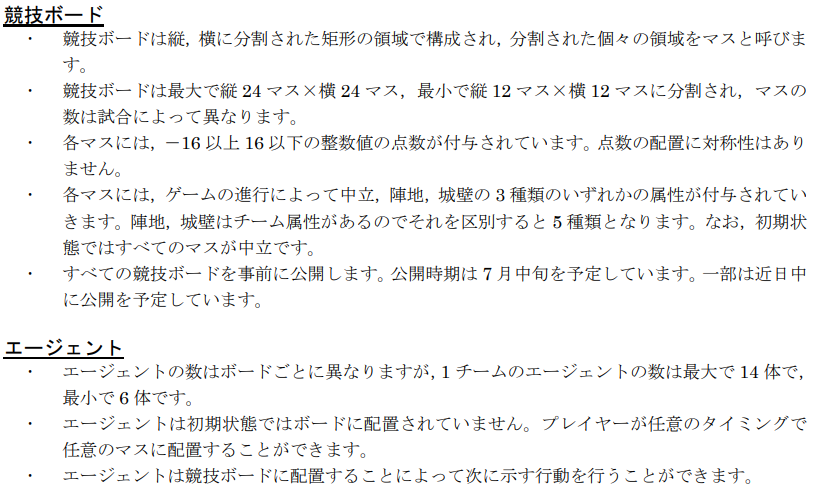
\includegraphics[scale=0.6]{memo_board.png}
            \caption{競技ボードの仕様(募集要項より)}
            \label{memoBoard}
        \end{figure}
        \begin{itemize}
            \item メンバ変数
            \begin{itemize}
                \item 盤面のサイズ
                \begin{itemize}
                    \item width $\cdots$ ボードの幅(12 - 24)
                    \item height $\cdots$ ボードの高さ(12 - 24)
                \end{itemize}
                \item エージェント数
                \begin{itemize}
                    \item agentNum $\cdots$ 各チームのエージェント数(6 - 14)
                \end{itemize}
                \item 盤面情報
                \begin {itemize}
                    \item field $\cdots$ 盤面の属性情報 (width*height, チャンネル数8)
                    各チャンネルとの関係
                    \begin{table}[H]
                        \label{tab1}
                        \centering
                        \caption{各チャンネルの割り当て}
                        \begin{tabular}{c|c}
                            チャンネル番号 & 割り当て \\ \hline
                            1 & 盤面の属性が中立か(yes:1 no:0)  \\ \hline
                            2 & 盤面の属性が自陣地か(yes:1 no:0) \\ \hline
                            3 & 盤面の属性が自城壁か(yes:1 no:0) \\ \hline
                            4 & 盤面の属性が敵陣地か(yes:1 no:0) \\ \hline
                            5 & 盤面の属性が敵城壁か(yes:1 no:0) \\ \hline
                            6 & 味方のエージェントがいるか(yes:1 no:0) \\ \hline
                            7 & 敵エージェントがいるか(yes:1 no:0) \\ \hline
                            8 & 盤面の得点(16 to -16) \\
                        \end{tabular}
                    \end{table}
                    *チャンネル分けは後に機械学習をするため
                \end{itemize}
                \item その他の情報
                \begin{itemize}
                    \item teamScore $\cdots$ 両チームの得点情報
                    \item agentCommand $\cdots$ エージェントの行動情報
                \end{itemize}
            \end{itemize}
            \item 関数一覧
            \begin{itemize}
                \item \_\_init\_\_ $\cdots$ 初期化関数 (in: width, height, agentNum / out: None)
                \item initField $\cdots$ 盤面を初期化 (in: None/ out: None)
                \item getField $\cdots$ 盤面の情報を返す (in: None/ out: field)
                \item printField $\cdots$ 盤面の情報を出力する (in: None/ out: None)
                \item setCommand $\cdots$ エージェントの行動情報を渡す (in: command/ out: None)
                \item updateAgents $\cdots$ エージェントの行動をする (in: None/ out: None)
                \item setAbility $\cdots$ 属性を塗り替える (in: width, height, ability/ out: None)
                \item judgeSurrounded $\cdots$ 囲み判定 (out: None)
            \end{itemize}
        \end{itemize}
}
\end{document}